\section{Operacje zmiennopozycyjne}
%%%%%%%%%%%%%%%%
\begin{frame}{Operacje zmiennopozycyjne}
    $x, y \in F$ \newline
    $x + y \in^? F$

    \begin{center}
    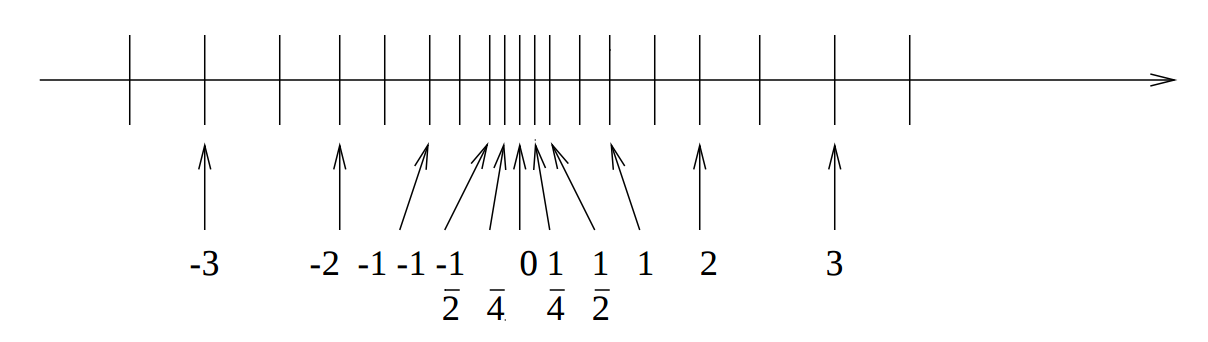
\includegraphics[width=0.8\linewidth]{img/2/2_1_axis}
    \end{center}
    System z powyższego rysunku: $\frac{5}{4} + \frac{3}{8} \notin F$ - ze względu na ,,gęstość'' elementów $F$.
\end{frame}
%%%%%%%%%%%%%%%%
\begin{frame}{Operacje zmiennopozycyjne}
    $\frac{7}{2} + \frac{7}{2} \notin F$ - {\it overflow}
    \vspace{.5cm}

    W większości komputerów: $x \oplus y = fl(x + y)$ dla $x + y$ z zakresu $F$

    $\oplus$ - dodawanie zmiennopozycyjne, \newline
    $fl(x)$ - reprezentacja zmiennoprzecinkowa 

    \[
    a + b = 2^{c_a} \cdot \left( m_a + m_b \cdot 2^{-(c_a-c_b)} \right) \Rightarrow
    \left\{ 
        \begin{array}{ll}
            |b| \le 1/2 \cdot 2^{-t} \cdot |a| \\
            fl(a + b) = a
        \end{array}
    \right.
    \]
\end{frame}
%%%%%%%%%%%%%%%%
\begin{frame}{Operacje zmiennopozycyjne}
    $x \cdot y$ rzadko $\in F$, bo:
    \begin{itemize}
    \item $x \cdot y$ ma $2 \cdot t$ lub $2 \cdot t - 1$ cyfr znaczących,
    \item {\it overflow} - bardziej prawdopodobny
    \item {\it underflow} - bardziej prawdopodobny
    \item $\oplus, \odot$
        \begin{itemize}
        \item są {\it przemienne}
        \item nie są {\it łączne}, {\it rozdzielne}
        \end{itemize}
    \end{itemize}
\end{frame}
%%%%%%%%%%%%%%%%
\begin{frame}{Operacje zmiennopozycyjne}
    Ogólnie:
    \[
    fl(a \square b) = rd(a \square b) = (a \square b) \cdot (1 + \varepsilon)
    \] \[
    \varepsilon = \varepsilon(a, b, \square), \varepsilon \le \beta^{1-t}
    \] \[
    \square = +, -, \cdot, /
    \]

    \begin{block}{Definicja}
        {\bf Maszynowe $\varepsilon$} - najmniejsza liczba zmiennoprzecinkowa, dla której jeszcze: \[
        1 \oplus \varepsilon > 1
        \]
        Wartość maszynowego $\epsilon$ określa precyzję obliczeń numerycznych wykonywanych na liczbach zmiennoprzecinkowych.
    \end{block}

    Zwykle wystarcza znajomość $\varepsilon' = 2^k \cdot \varepsilon, k \approx 1, 2, 3, ...$ $\rightarrow$ fragment progr. $\varepsilon$
\end{frame}
%%%%%%%%%%%%%%%%
